% !TeX root = Protokoll.tex
\subsection{Energieaufspaltung}
Ein Atom besitzt verschiedene möglichkeiten wie sich deren Energieniveaus aufteilen. Dazu wird zunächst der Fall eines Atoms mit verschwindenden Kernspins behandelt.
Der Gesamtdrehimpuls der freien Elektronen eines Atoms $\vec{J}$ erzeugt ein magnetisches Moment $\vec{\mu}_J $ deren Zusammenhang gegeben ist durch
\begin{align}
	\vec{\mu}_J=&-g_J \cdot \mu_B \cdot \vec{J}\\
	\Rightarrow |\vec{\mu}_J|=&\hspace{1em} g_J\cdot\mu_B\cdot\sqrt{J\cdot(J+1)}.
\end{align}
Darin ist $g_J$ der Landé-Faktor und $\mu_B$ das Bohrsche Magneton.
Mithilfe des Landé-Faktors wird berücksichtigt das sich der Gesamtdrehimpuls aus dem Bahndrehimpuls $\vec{L}$ und dem Spin $\vec{S}$ zusammen setzt.
Für deren magnetischen Momente $\vec{\mu}_{L/S}$ gilt 
\begin{align}
	|\vec{\mu}_L|=&\mu_B\sqrt{L\cdot(L+1)}\\
	&\text{und}\nonumber\\
	|\vec{\mu}_S|=& g_S\cdot\mu_B\sqrt{S\cdot(S+1)}.
\end{align}
Mithilfe der vektoriellen Gleichung
\begin{align}
	\vec{\mu}_L=&\vec{\mu}_L+\vec{\mu}_S\\
	\Rightarrow |\vec{\mu}_J|=&|\vec{\mu}_L|\cos(\beta)+|\vec{\mu}_S|\cos(\alpha)
\end{align}
lässt sich unter zu Hilfe nahme des Kosinussatzes und dem aufgespannten Dreieck von $\vec{J},\ \vec{L}$ und $\vec{S}$ eine Formel für $g_J$ herleiten.
\begin{align}
	g_J =\frac{(g_s + 1)\cdot J \cdot (J+1)+(g_S-1)\cdot\left[S\cdot(S+1)-L\cdot(L+1)\right]}{2\cdot J \cdot (J+1)}
	\label{eq:lande_faktor_gj}
\end{align}
Wird nun ein äußeres Magnetfeld $B$ angelegt, so tritt eine Aufspaltung der Energieniveaus auf.
Dabei ist die Energie der magnetischen Wechselwirkung gegeben als 
\begin{align}
	U_{\text{mag}}=-\vec{\mu}_J\cdot \vec{B}=M_J\cdot g_J\cdot \mu_B\cdot B.\label{eq:magEnergie}
\end{align}
Darin ist $M_J\in[-J, -J+1,\hdots,J-1,J]$, dies Folgt aus der Richtungsquantelung.
Dieser Effekt wird Zeeman-Effekt genannt.
Bis jetzt wurde angenommen das der Kern einen Kernspin von Null hat.
Nun wird der Fall betrachtet das der Kernspin von Null verschieden ist.
Der Gesamtdrehimpuls der Elektronhülle $\vec{J}$ und der Kernspin $\vec{I}$ koppeln bei hinreichend schwachen Magnetfeld vektoriell aneinander zum Gesamtdrehimpuls der Systems $\vec{F}$.
\begin{align}
	\vec{F}=\vec{J}+\vec{I}
\end{align}
Die Energieniveaus spalten sich jetzt in die Hyperfeinstruktur auf und bilden $2J+1$ oder $2I+1$ Niveaus, je nach dem ob I größer ist als J oder anders herum.
Die Aufspaltung eines einzelnen Niveaus kann mithilfe der Quantenzahl $F$ bestimmt werden, die von $I+J$ bis $|I-J|$ läuft.
Durchs anlegen eines externen kleinen Magnetfeldes wird die Hyperfeinstruktur in $2F+1$ Zeeman-Nivaus aufgespalten.
Ein Beispiel ist in \cref{BeispielAufspaltung} Dargestellt.
\begin{figure}[h!]
	\centering
	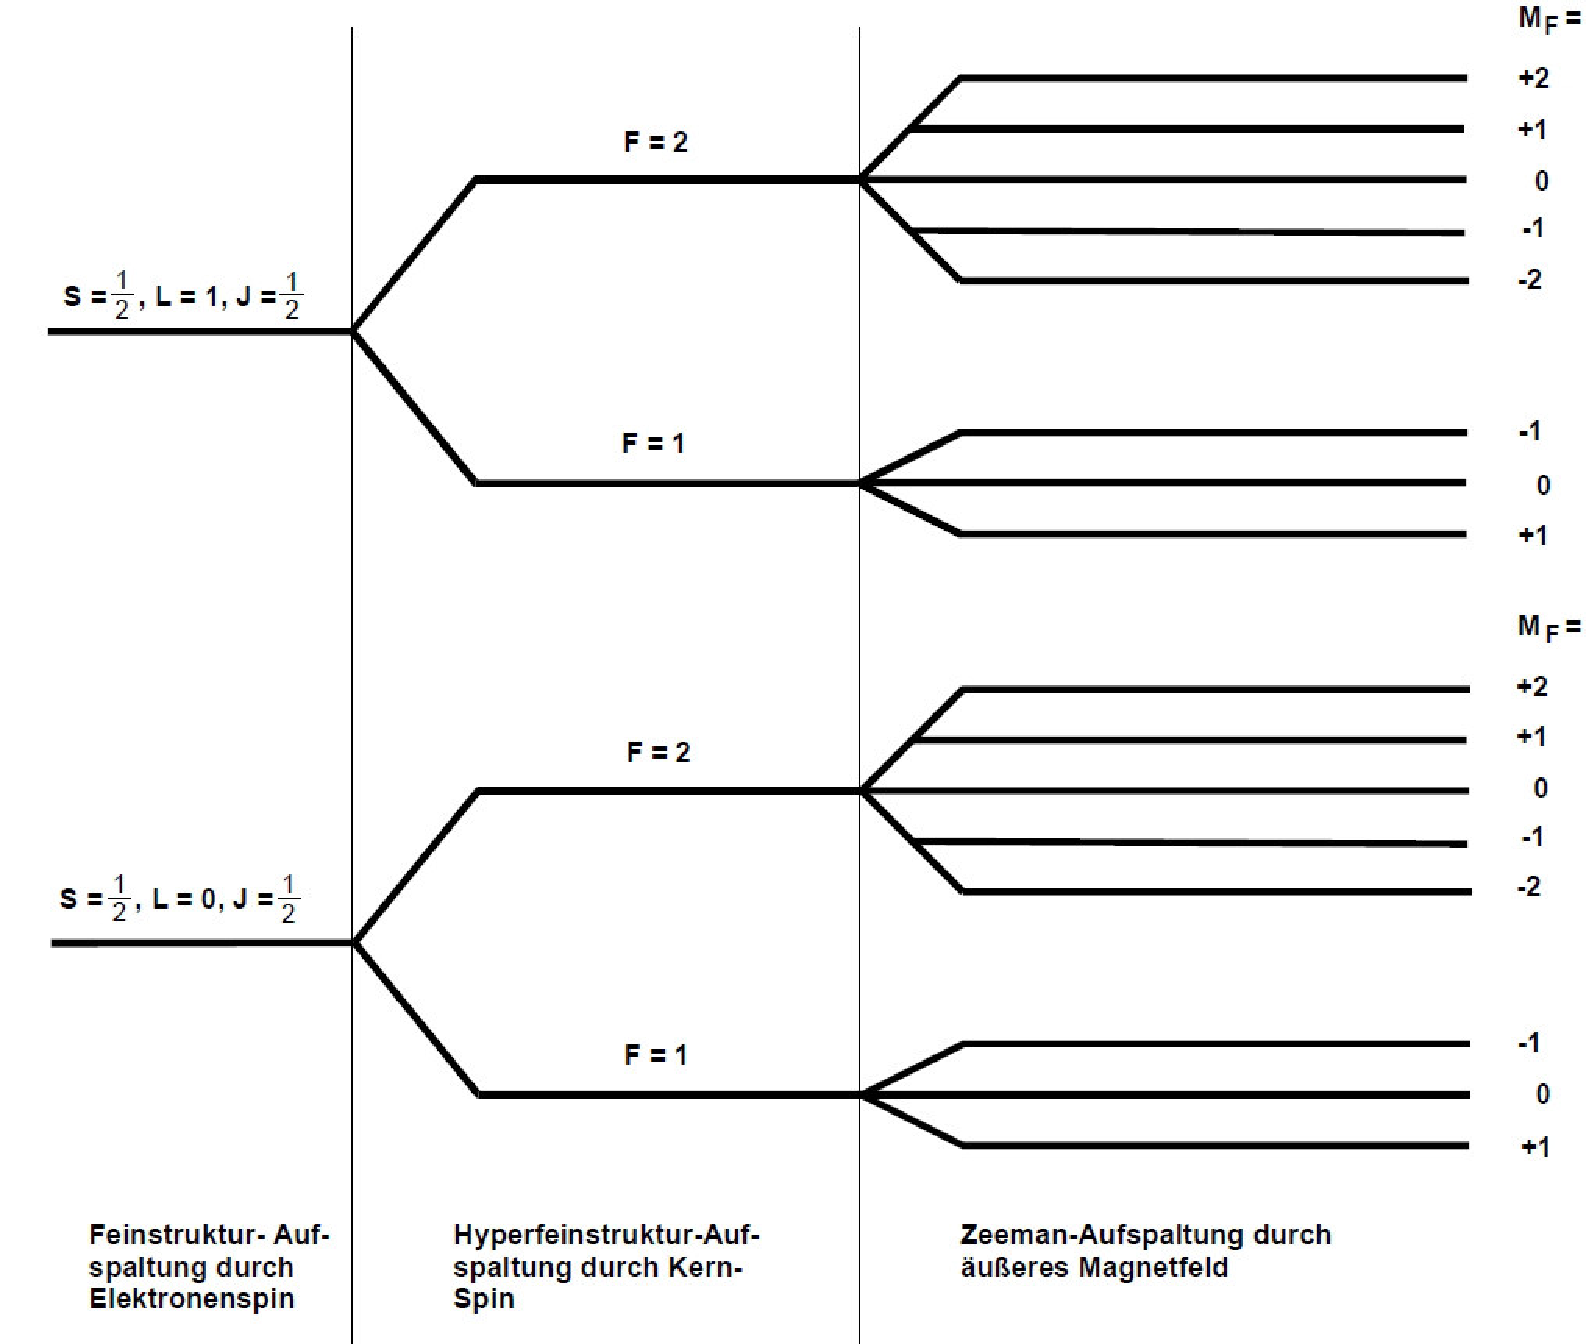
\includegraphics[width = 0.8\textwidth]{../Grafiken/BeispielAlkali.pdf}
	\caption{Beispiel für die Aufspaltungen durch Elektronenspin, Kernspin und äußeren Magnetfeld anhand eines Alkali-Atoms mit $I=\frac{3}{2}$ und $J=\frac{1}{2}$.\cite{V21}}\label{BeispielAufspaltung}
\end{figure}\\
Die Differenz von zwei benachbarten Energieniveaus ist gegeben durch
\begin{align}
	U_\text{HF}=g_F\mu_BB.
\end{align}
Der Landé-Faktor für die Zeeman-Aufspaltung, lässt sich mithilfe von
\begin{align}
	|\vec{\mu}_B|&=g_F \cdot \mu_B \sqrt{F \cdot (F+1)}\\
	&=g_J \cdot \mu_B\sqrt{J \cdot (J+1)} \cdot \cos\left(\measuredangle(\vec{J},\vec{F})\right) + g_I \cdot \mu_K \sqrt{I\cdot(I+1)}\cdot \cos\left(\measuredangle(\vec{I,\vec{F}})\right)\nonumber
\end{align}
bestimmen. Dabei ist $\mu_K$ das magnetische Moment des Kerns, allerdings ist die Masse des Kerns viel größer, weshalb $\mu_K \ll \mu_B$ gilt. Dadurch lässt sich der Landé-Faktor bestimmen zu
\begin{align}
	g_F\approx g_J\frac{F\cdot(F+1)+J\cdot(J+1)-I(I+1)}{2F\cdot(F+1)},
	\label{eq:lande_faktor_gf}
\end{align}
wobei wieder der Kosinussatz verwendet wurde.

\subsection{Optisches Pumpen}
In einem isolierten Atom, sind die Zustände niedrigster Energie, aufgrund des Pauliprinzips vollständig besetzt.
In höheren Zuständen kann das Verhältnis zweier Besetzungszahlen $N_{1/2}$ mithilfe der Boltzmannstatistik beschrieben werden
\begin{align}
	\frac{N_2}{N_1}=\frac{g_2}{g_1}\frac{\exp(-W_2/k_BT)}{\exp(-W_1/k_BT)}.\label{eq:ZustandsVerteilung}
\end{align}
Dabei ist $W_i$ die Energie zur Besetzungszahl $N_i$, $T$ die Gleichgewichtstemperatur und $k_B$ die Boltzmannkonstante. 
Die $g_i$ sind die statistischen Gewichte.
Weil $W_2>W_1$ ist, kann daraus abgelesen werden das die Zustandszahl $N_1$ mehr besetzt ist als die Zustandszahl $N_2$.
Mithilfe des optischen Pumpens, kann eine Abweichung von Gleichung \eqref{eq:ZustandsVerteilung} erzeugt werden.
Es kann sogar der Zustand der Besetzungsinversion auftreten $N_2 > N_1$.
Die Energie die ein Lichtquant haben muss um von dem Atom absorbiert zu werden muss
\begin{align}
	hf=W_2-W_1
\end{align}
sein. 
Das ist die gleiche Energie wie die eines emittierten Photons.\\
\begin{figure}[h!]
	\centering
	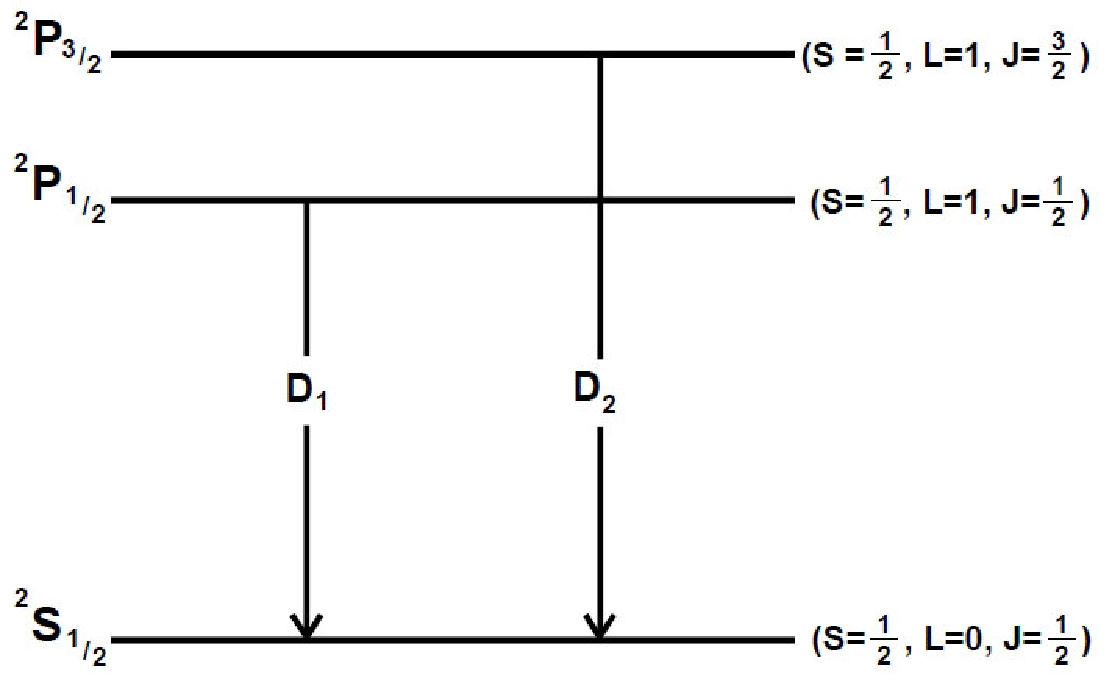
\includegraphics[width = 0.49\textwidth, height = 0.3\textwidth]{../Grafiken/Alkali-Spektrum.pdf}
	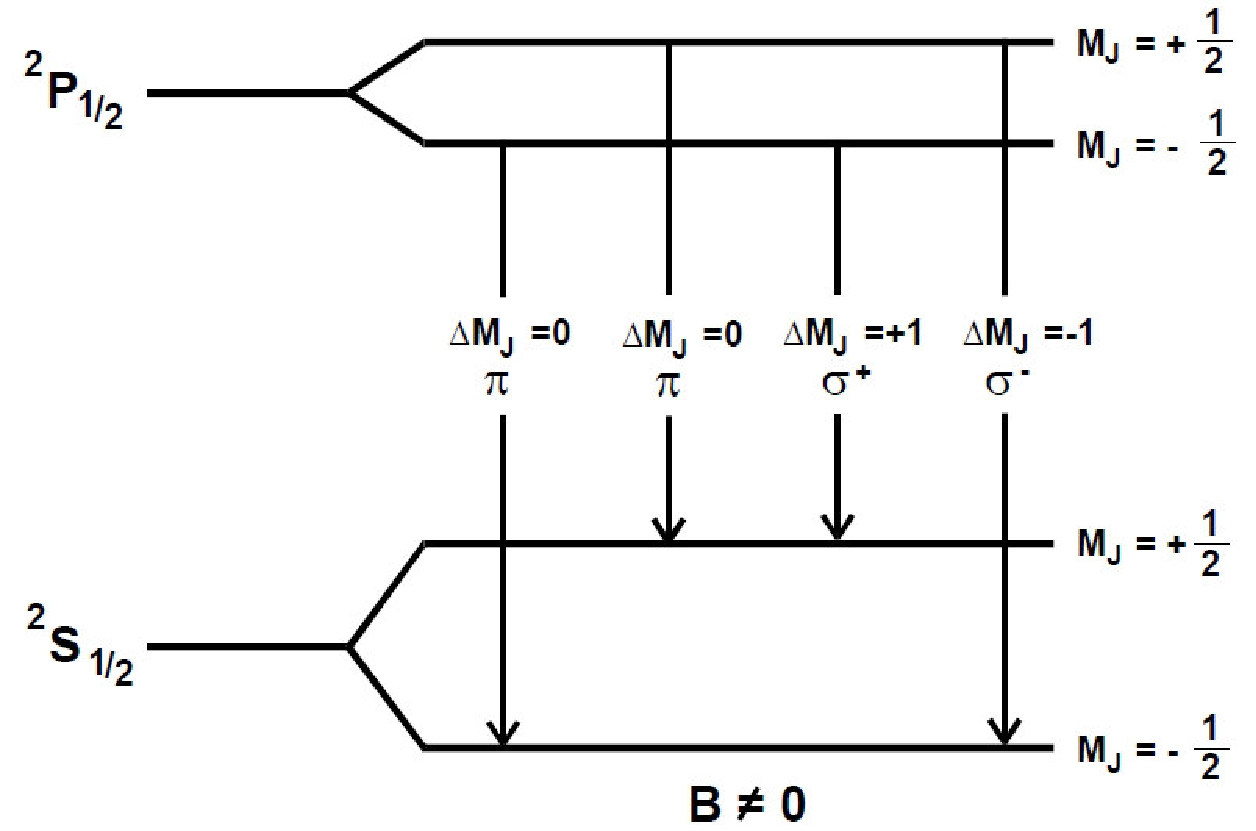
\includegraphics[width = 0.49\textwidth, height = 0.3\textwidth]{../Grafiken/ZeemanAufspaltung.pdf}
	\caption{Hier ist die Dublettstruktur des Aklali-Spektrums dargestellt und die Dazugehörigen Quantenzahlen, sowie die Zeeman-Aufspaltung des Grundniveaus und des ersten angeregten Zustandes und deren Übergänge.\cite{V21}}\label{fig:Aufspaltung}
\end{figure}
Es wird zunächst das Beispiel des Alkali-Atoms behandelt, weil dieses ein freies Elektron besitzt und keinen Kernspin.
Dadurch hat es den Grundzustand ${}^2S_{{}^1\!/\!_2}$ und die zwei erst angeregte Zustände ${}^2P_{{}^1\!/\!_2}$ und ${}^2S_{{}^3\!/\!_2}$.
Es sind 2 optische Übergänge möglich, $D_1$ und $D_2$.
Die Zustände ${}^2S_{{}^1\!/\!_2}$ und ${}^2P_{{}^1\!/\!_2}$ haben $J={}^1\!/\!_2$. 
Daraus folgt das die Aufspaltung $M_J=\pm^1\!/\!_2$ ist und die daraus folgende Differenz $\Delta M_J = 0 ,\pm1$. Diese Übergänge sind in \cref{fig:Aufspaltung} dargestellt.\\
Der Übergang $\sigma^+$ ($\Delta M_J=+1$) entspricht rechtszirkular-polarisiertes Licht, das bedeutet das der Spin der Lichtquanten antiparallel zur Ausbreitungsrichtung ist und bei dem $\sigma^-$-Übergang ($\Delta M_J=-1$) steht der Spin parallel. 
Die Lichtquanten sind bei dem $\pi$-Übergang ($\Delta M_J=0$) hingegen linear polarisiert. 
Dabei werden die $\sigma$-Übergänge entlang des Magnetfeldes abgestrahlt und die $\pi$-Übergänge senkrecht dazu.
Wird nun Gas aus diesem Alkali-Atom im thermischen Gleichgewicht durch zirkularpolarisiertes $D_1$-Licht angeregt, entlang des Magnetfeldes ($\Delta M_J=\pm1$), tritt nur der Übergang von ${}^2S_{^1\!/\!_2}$, $M_J=-^1\!/\!_2$ nach ${}^2P_{^1\!/\!_2}$, $M_J=+^1\!/\!_2$ auf. Durch spontane Emission tritt der Übergang von ${}^2P_{^1\!/\!_2}$, $M_J=+^1\!/\!_2$ sowohl nach ${}^2S_{^1\!/\!_2}$ $M_J=-^1\!/\!_2$ als aber auch nach ${}^2S_{^1\!/\!_2}$ $M_J=+^1\!/\!_2$. 
Dies sorgt dafür das der höhere Zustand ${}^2S_{^1\!/\!_2}$, $M_J=+^1\!/\!_2$ mehr besetzt ist als Zustand ${}^2S_{^1\!/\!_2}$, $M_J=-^1\!/\!_2$.
Wenn der energetisch niedrigere Zustand ${}^2S_{^1\!/\!_2}$ $M_J=-^1\!/\!_2$ weniger besetzt ist, wird das $D_1$-Licht nicht mehr absorbiert und kann somit mit vollständig gemessen werden.
Im Energiebereich des Zeeman-Niveaus, tritt spontane Emission praktisch nicht auf, dies bedeutet das überwiegend induzierte Emission eine Rolle spielen.
\newpage
\subsection{Resonanzstellen}
\begin{figure}[h!]
	\centering
	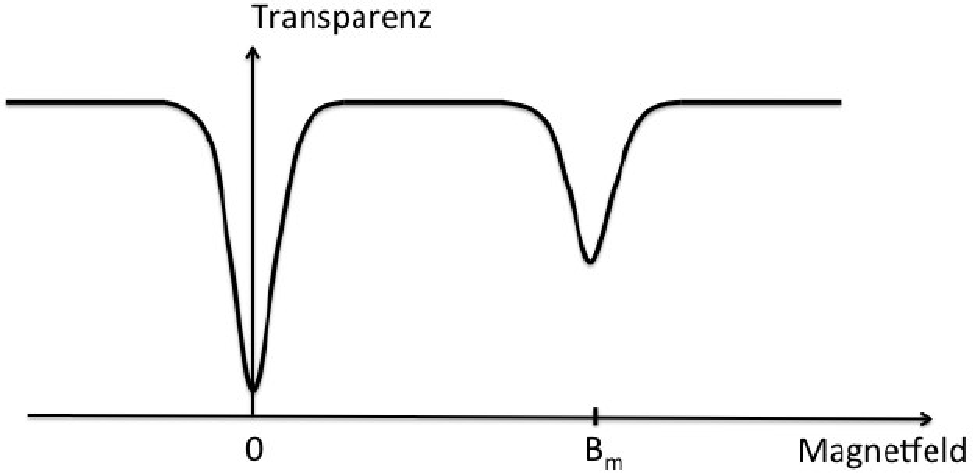
\includegraphics[width = 0.75\textwidth]{../Grafiken/Resonanz.pdf}
	\caption{Die Darstellung der Transparenz eines Alkaliatoms in Abhängigkeit des angelegten Magnetenfelds.\cite{V21}}\label{fit:Resonanz}
\end{figure}
Es gibt für ein Alkali-Atom 2 Resonanzstellen.
Als erstes gibt es eine bei $B=0$, dies kann dadurch erklärt werden, dass keine Zeeman-Aufspaltung stattfindet und somit auch kein optisches Pumpen möglich ist.
Hier mit können die Einflüsse des Erdmagnetfeldes bestimmt und ausgeglichen werden.
Durch angeschalteten Magnetfeld wird das Pumpen begonnen und somit die Besetzungsinversion herbeigeführt.
Wenn nun die Energie eines Photons gleich der Energiedifferenz der Zeeman-Aufspaltung ist, tritt wieder induzierte Emission auf, dass zur folge hat das sich das ${}^2S_{{}^1\!/\!_2}$, $M=-^1\!/\!_2$ Niveau füllt.
Die Magnetfeldstärke der Resonanzstelle ist dabei durch
\begin{align}
	\notag
	hf = U_\text{HF} =& \mu_B\cdot g_J\cdot B_\text{Res}\\
	\Rightarrow B_\text{Res}=&\frac{4\pi m_0}{e_0g_J}f
	\label{eq:gerade_magnetfeld_frequenz}
\end{align}
gegeben.
\newpage
\subsection{Verallgemeinerung für nicht verschwindenden Kernspin}
\begin{figure}[h!]
	\centering
	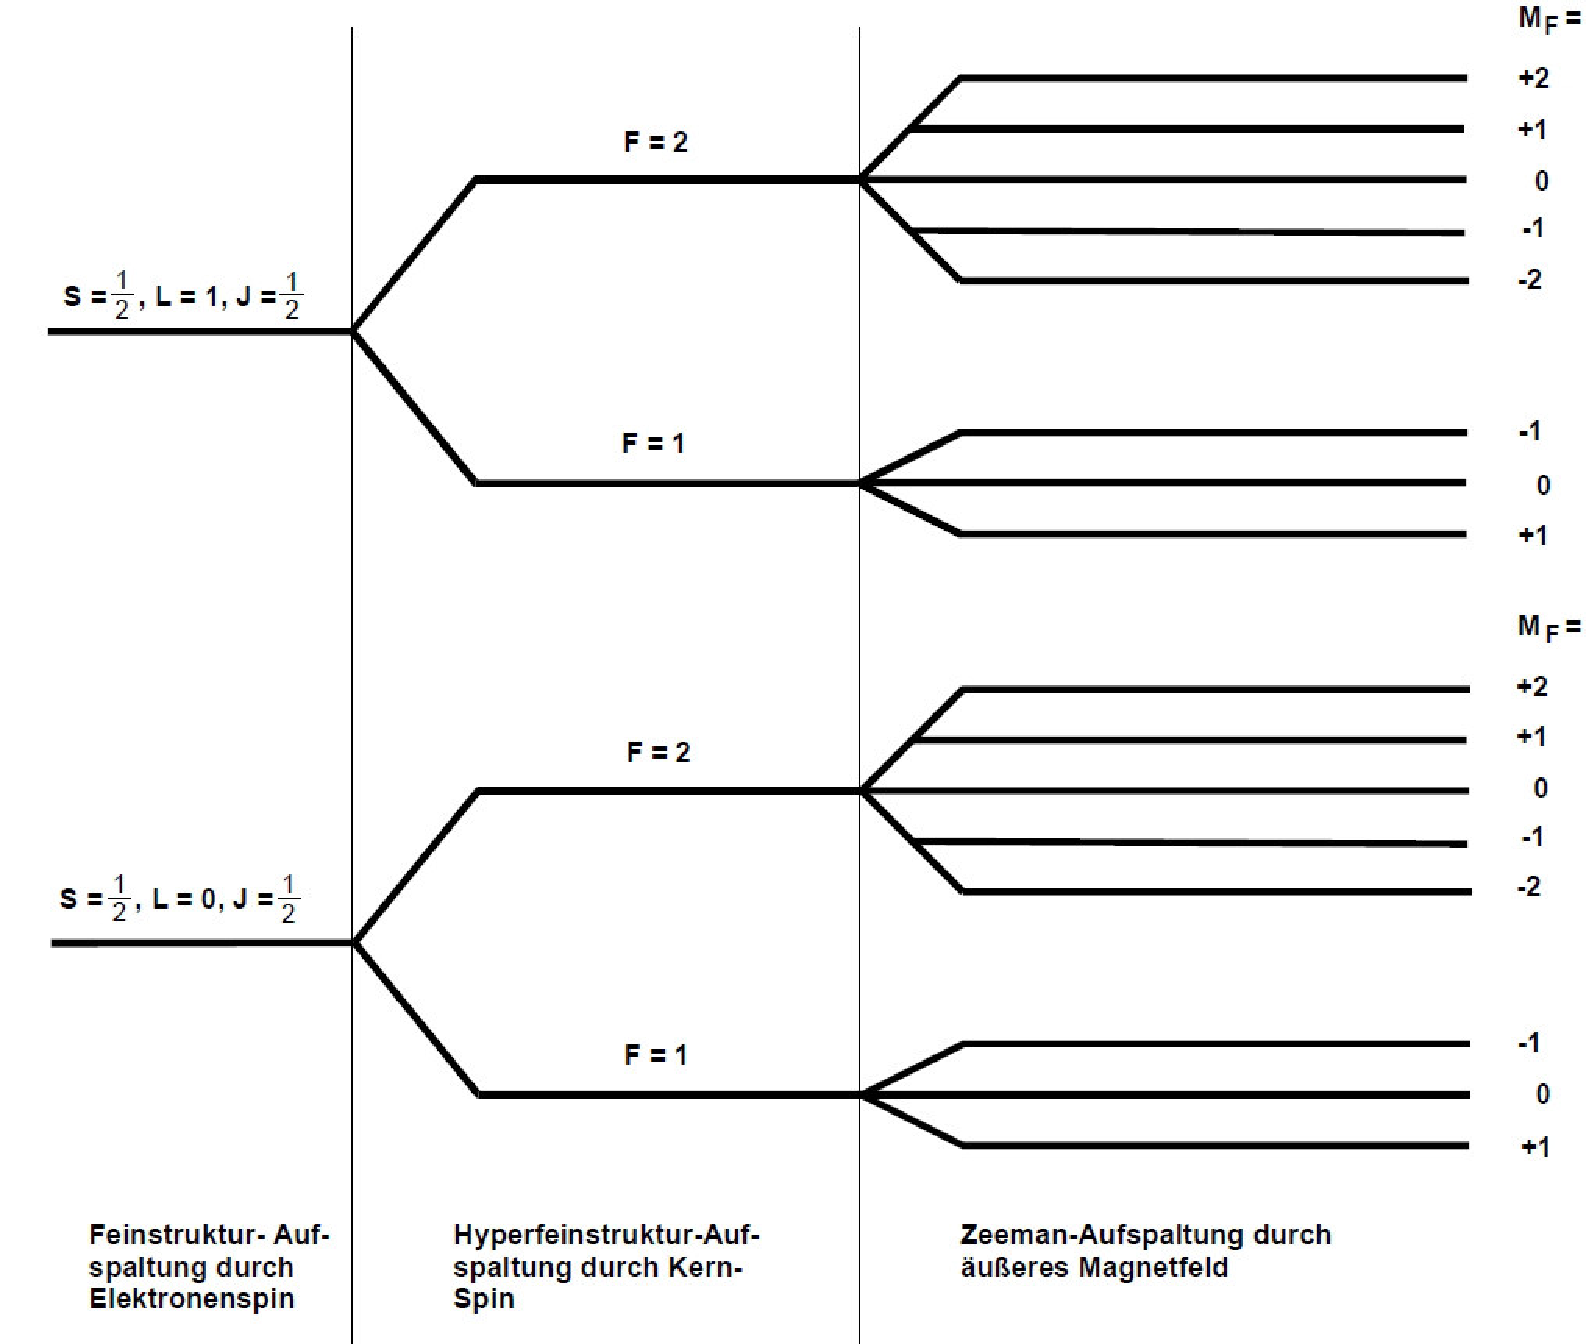
\includegraphics[width = 0.8\textwidth]{../Grafiken/BeispielAlkali.pdf}
	\caption{Energieaufspaltung für ein Atom mit Kernspin ungleich null.\cite{V21}}\label{fig:Kernspin}
\end{figure}
Durch den von null verschiedenen Kernspin wird die Aufspaltung in den Zeeman-Niveaus umfangreicher, wie in \cref{fig:Kernspin} für $I={}^3\!/\!_2$ dargestellt.
Wird auf das System zirkularpolarisiertes Licht gestrahlt, sind nur Übergänge mit $\Delta M_F=+1$ möglich.
Dies sorgt dafür, dass keine Übergänge von $F=2$, $M_F=+2$ möglich sind, weil kein $M_F=+3$ existiert.
Dies hat zur folge, das mit der Zeit die Besetzungszahl zunehmen wird, weil durch spontane Emission der zustand weiter besetzt werden kann.
Das sorgt dafür, dass das Grundniveau leer gepumpt wird.
Wird nun ein Magnetfeld mit der Magnetfeldstärke der Resonanzstelle angelegt, wird auch hier das Niveau sich leeren und der Grundzustand kann wieder leer gepumpt werden.

\newpage
\subsection{Quadratischer Zeeman-Effekt}
Bei höheren Magnetfeldern müssen Terme höherer Ordnung mit berücksichtigt werden für $U_\text{HF}$.
Druch lösen der Eigenwertgleichung 
\begin{align}
	H\psi = U\psi
\end{align}
unter Berücksichtigung der magnetischen Momente $\vec{\mu}_J$ und $\vec{\mu}_I$, wird die Energie abhängig von der Quantenzahl $M_F$.
Die Energie lässt sich schreiben als
\begin{align}
	U_\text{HF}= g_F\mu_B+g_F^2\mu_B^2B^2\frac{1-2M_F}{\Delta E_\text{Hy}}-\cdots,
	\label{eq:zeeman_effekt_quadratisch}
\end{align}
wobei $\Delta E_\text{Hy}$ die Energiedifferenz der Niveaus $F$ und $F+1$ ist.
\subsection{Transiente Effekte}
Bis jetzt wurden nur konstante Magnetfelder Betrachtet.
Nun wird der Fall für sich Periodisch ändernde Magnetfelder behandelt.
Das Magnetfeld und die Frequenz seien auf die Resonanzstelle eingestellt.
Dann ist die Frequenz gegeben als 
\begin{align}
	\omega_0=2\pi f_0=g_F\frac{\mu_B}{h}B_0=\gamma B_0
\end{align}
wobei $\gamma$ das gyromagnetische Verhältnis ist und als 
\begin{align}
	\gamma=g_F\frac{\mu_B}{h}
\end{align}
definiert ist.
Durch lösen einer klassischen Differentialgleichung für ein stationäres Magnetfeld $B$ und einem senkrecht dazu rotierenden Magnetfeld $B_{RF}$, lässt sich zeigen das sich das Problem als Summe von einem konstanten Magnetfeld und dem Magnetfeld ${}^\omega\!/\!_\gamma$ auffassen lässt, dadurch kann
\begin{align}
	B_\text{eff}=B+\frac{\omega}{\gamma}
\end{align}
definieren.
Es lässt sich für den Resonanzfall zeigen, dass $|B_\text{eff}| =B_\text{RF}$ ist.
Daraus folgt, dass es sich mit der Larmor-Frequenz $f=\gamma_\text{RF}$ Rotiert.
Die resultierende Periode ist somit $T=^1 \!\! /\!_{\gamma B_{RF}}$.
Für zwei Isotope bei resonanten Magnetfeld gilt somit
\begin{align}
	\frac{T_{87}}{T_{85}}=\frac{\gamma_{85}}{\gamma_{87}}.
\end{align}